\documentclass[french,nochapter,11pt]{rapportUB}  
% Options french (1-) ou english (2-)
%    1- si vous rédigez en français (chargement du package [french]{babel})
%    2- si vous rédigez en anglais (chargement du package [english]{babel})
% Options chapter (1-) ou nochapter (2-)
%    1- la commande \chapter peut être utilisée dans le document (la classe report est chargée)
%    2- la commande \chapter NE peut PAS être utilisée dans le document (la classe article est chargée)
% Options 10pt ou 11pt ou 12pt (taille des caractères)
% Option nologo (à utiliser seulement si vous ne souhaitez pas afficher le logo de l'université sur la première page / le logo doit être dans le même dossier que votre fichier tex et s'appeler logo (l'extension n'a pas d'importance)
%
% Les options par défaut sont french, nochapter,11pt

\college{Collège Sciences et Technologies}
\uf{UF Mathématiques et Interactions - Informatique}
\program{Licence Mathématiques Informarique} %A remplir
\course{Projet tutoré} %A remplir
\academicyear{2020 -- 2021} %A remplir
\author{ %A remplir
  Corentin Banier
  \\
  Maher Karboul
}

%Paquetages additionnels
\usepackage{placeins}
\usepackage{multirow}
\usepackage{framed}
%Pour gérer la bibliographie
\usepackage[backend=bibtex,style=authoryear]{biblatex}
\addbibresource{biblio.bib}
\DeclareDelimFormat{nameyeardelim}{\addcomma\space}

%Déclaration d'un nouvel opérateur
\DeclareMathOperator*{\argmin}{arg\,min}
\DeclareMathOperator*{\argmax}{arg\,max}
%bib pour les matrices
\usepackage{amsmath}
\usepackage{arydshln}
\usepackage{amsfonts}
\usepackage{stmaryrd}
\usepackage{listings}
\lstset{
  literate=
  {á}{{\'a}}1 {é}{{\'e}}1 {í}{{\'i}}1 {ó}{{\'o}}1 {ú}{{\'u}}1
  {Á}{{\'A}}1 {É}{{\'E}}1 {Í}{{\'I}}1 {Ó}{{\'O}}1 {Ú}{{\'U}}1
  {à}{{\`a}}1 {è}{{\`e}}1 {ì}{{\`i}}1 {ò}{{\`o}}1 {ù}{{\`u}}1
  {À}{{\`A}}1 {È}{{\'E}}1 {Ì}{{\`I}}1 {Ò}{{\`O}}1 {Ù}{{\`U}}1
  {ä}{{\"a}}1 {ë}{{\"e}}1 {ï}{{\"i}}1 {ö}{{\"o}}1 {ü}{{\"u}}1
  {Ä}{{\"A}}1 {Ë}{{\"E}}1 {Ï}{{\"I}}1 {Ö}{{\"O}}1 {Ü}{{\"U}}1
  {â}{{\^a}}1 {ê}{{\^e}}1 {î}{{\^i}}1 {ô}{{\^o}}1 {û}{{\^u}}1
  {Â}{{\^A}}1 {Ê}{{\^E}}1 {Î}{{\^I}}1 {Ô}{{\^O}}1 {Û}{{\^U}}1
  {œ}{{\oe}}1 {Œ}{{\OE}}1 {æ}{{\ae}}1 {Æ}{{\AE}}1 {ß}{{\ss}}1
  {ű}{{\H{u}}}1 {Ű}{{\H{U}}}1 {ő}{{\H{o}}}1 {Ő}{{\H{O}}}1
  {ç}{{\c c}}1 {Ç}{{\c C}}1 {ø}{{\o}}1 {å}{{\r a}}1 {Å}{{\r A}}1
  {€}{{\EUR}}1 {£}{{\pounds}}1
}

\begin{document}

\title{Codes LDPC}

\maketitle

\begin{center}
\tableofcontents %affichage de la table des matières
\clearpage
\end{center}

%-----------------------------------------------------
% IMPORTANT : A décommenter pour ajouter l'engagement de non plagiat au rapport.
%\nonplagiat{Prenom1 Nom1}[Prenom2 Nom2][Prenom3 Nom3]
%-----------------------------------------------------


\section{Introduction}
\label{sec:introduction}
La conception des codes LDPC binaires avec un faible poids d'erreurs demeurre un problème non entiérement résolu. 
Les codes LDPC (Low Density Parity Check) sont des codes linéaires correcteurs d'erreurs qui assurent la transmission d'informations. 
Ils forment une classe de codes en bloc qui se caractérisent par une matrice de contrôle creuse. Ils ont été décrits pour la première 
fois dans la thèse de Gallager au début des années 60. Dans ce travail, nous allons étudier comment fabriquer des instances de ce code 
notamment avec le modèle de Gallager. Puis, nous comprendrons comment décoder des codes LDPC, on essaiera d'optimiser ce dernier en limitant
le nombre d'équation à satisfaire par un mot de code erroné.\vspace{0.4cm}\newline
Le rapport est organisé de la manière suivante; la section \ref{sec:fabrication} présente les étapes de fabrication d'un code LDPC 
ainsi qu'une matrice de contrôle qui répond à des conditions bien spécifiques. La section \ref{sec:algo} présente l'algorithme 
détaillé de décodage LDPC. La section \ref{sec:exp} est dédiée aux expériences pratiques qu'on a effectué durant l'implémentation 
de l'algorithme. Enfin, la section \ref{sec:conclusion} sera notre conclusion sur le projet.\vspace{0.4cm}\newline
Avant tout, nous allons introduire la notion de code correcteur d'erreur(s).\vspace{0.7cm}\newline
\textbf{\underline{PS:}} L'ensemble du code réalisé durant le projet est disponible sur le dépôt GitHub à l'adresse suivante : \url{https://github.com/cbanier/codes-LDPC}
\newline Nous utilisons le module \textsc{numpy}.
\clearpage

%-----------------------------------------------------
%-----------------------------------------------------

\section{Codes correcteurs}
Lors de la transmission d'une information, des erreurs peuvent se produirent. Cette problématique de correction des erreurs de transmission est 
très importante dans notre monde connecté, qu'il s'agisse des communications entre ordinateurs par internet, des conversations téléphoniques etc...\newline
Un code correcteur, souvent désigné par le sigle anglais ECC (Error-correcting code), est une technique de codage basée sur la redondance.\newline
Un code est une application injective $\Phi:\{0,1\}^k \rightarrow \{0,1\}^n $.\newline
Le paramètre k est appelé la \textbf{dimension} du code $\Phi$ et le paramètre n est appelé la \textbf{longueur} du code : on dit que $\Phi$ est un 
code de paramètres (k,n).\vspace{0.4cm}\newline
Soit $\Phi$ un code d'image C.\newline
On appelle \textbf{capacité de correction} de $\Phi$ le plus grand entier $e_c$ tel qu'on soit toujours capable de corriger $e_c$ erreurs ou moins. \newline
On appelle \textbf{distance minimale} de $\Phi$ et on note $d_c$ la plus petite distance non nulle entre deux mots de code. \newline
Ainsi, on a \textbf{$e_c = $} $\frac{d_c-1}{2}$\vspace{0.4cm}\newline
Parmi les exemples de codes correcteurs, on peut citer les codes de répétition, les codes carré et on encore les codes LDPC.
%-----------------------------------------------------
\subsection{Code de répétition}
Le code de répétition se résume par transmettre le message deux fois pour s'assurer contre les erreurs. Par exemple, Alice veut transmettre un mot de quatre bits à Bob. 
\begin{tabbing}
\hspace{5cm}\textbf{m=0111} \newline
\end{tabbing}
Elle va donc envoyer le mot codé
\begin{tabbing}
    \hspace{5cm}\textbf{c=01110111}
\end{tabbing}
le mot reçu par Bob sera noté y. Par exemple, si Bob reçoit
\begin{tabbing}
    \hspace{5cm}\textbf{y=01110110}
\end{tabbing}
Il peut constater qu'une erreur, au moins, s'est produite. Il peut dire que l'erreur est soit sur le quatrième ou le huitième bit.
%-----------------------------------------------------
\subsection{Code carré}
On suppose que Alice veut transmettre le mot de quatre bits, \textbf{m=$x_1$$x_2$$x_3$$x_4$}. Pour cela, elle l'écrit dans un carré de la façon suivante \newline
\begin{tabbing}
  \hspace{5cm} $x_1$ $x_2$ \\
  \hspace{5cm} $x_3$ $x_4$
\end{tabbing}
Elle rajoute ensuite les bits, dits de parité, $p_1$,$p_2$,$p_3$,$p_4$ de sorte qu'il y ait un nombre pair de 1 sur chaque ligne et chaque colonne. \newline
La somme sur chaque ligne et chaque colonne est 0 modulo 2. \newline
Le code sera affiché de cette façon :
\begin{tabbing}
  \hspace{5cm} $x_1$ $x_2$ $p_1$ \\
  \hspace{5cm} $x_3$ $x_4$ $p_2$ \\
  \hspace{5cm} $p_3$ $p_4$
\end{tabbing}
Le mot codé envoyé par Alice est : 
\begin{tabbing}
  \hspace{5cm}\textbf{c=$x_1$$x_2$$x_3$$x_4$$p_1$$p_2$$p_3$$p_4$}
\end{tabbing}
On prend l'exemple suivant : \textbf{m=0011}, la première étape est :
\begin{tabbing}
  \hspace{5cm}\textbf{0 0} \\
  \hspace{5cm}\textbf{1 1}
\end{tabbing}
En rajoutant les bits de parité, on obtient
\begin{tabbing}
  \hspace{5cm}\textbf{0 0 0}\\
  \hspace{5cm}\textbf{1 1 0 }\\
  \hspace{5cm}\textbf{1 1}
\end{tabbing}
Le mot codé est donc \textbf{c=00110011}
%-----------------------------------------------------
\subsection{Code linéaire}
\textbf{Définition:} Soient $\mathbb{F_q}$ un corps fini à q éléments, n$\geq$1 un entier. On dit que C $\subset$ $\mathbb{F_q}^n$ est un code linéaire si C est un sous-espace vectoriel de $\mathbb{F_q}^n$. Comme tout espace vectoriel, C a une dimension k. \newline
La construction de ce type de code est : $\phi$: $\mathbb{F_q}^k$ $\to$ $\mathbb{F_q}^n$. D'où C=Im$\phi$ est un sous espace-vectoriel de $\mathbb{F_q}^n$, et par le théorème du rang dimC = k. \newline
\textbf{Exemple de code linéaire:} Le code carré. 
%-----------------------------------------------------
\subsection{Matrice génératrice}
\textbf{Définition d'une matrice génératrice:} Soit C $\subset$ $\mathbb{F_q}^n$ un code linéaire de dimension k. Une matrice G dont les lignes forment une forme de C s'appelle \textbf{matrice génératrice} de C. Elle aura donc k lignes et n colonnes. \newline
\textbf{Exemple:} \textbf{Le code carré:}On rappelle que c'est l'image de l'application linéaire injective \newline 
 
$\begin{array}{cccc}
  \phi :  \mathcal{F}_2^4 \to  \mathcal{F}_2^8 \cr
(x_1,x_2,x_3,x_4) \mapsto (x_1,x_2,x_3,x_4,x_1+x_2,x_3+x_4,x_1+x_3,x_2+x_4)
\end{array}$
\newline
Une base de l'image est l'image d'une base. Par exemple l'image de la base  canonique. \newline
Donc $\phi(1000)$ = \textbf{10001010} \newline
$\phi(0100)$ = \textbf{01001001} . \newline
De même pour $\phi(0010)$=\textbf{00100110} \newline
Et aussi $\phi(0001)$ = \textbf{00010101} \newline
On obtient donc une matrice génératrice
$$G=
\begin{pmatrix}
  1 & 0 & 0 & 0 & 1 & 0 & 1 & 0  \\
  0 & 1 & 0 & 0 & 1 & 0 & 0 & 1  \\
  0 & 0 & 1 & 0 & 0 & 1 & 1 & 0  \\
  0 & 0 & 0 & 1 & 0 & 1 & 0 & 1 
  
  
\end{pmatrix}
\quad
$$
%-----------------------------------------------------
\subsection{Matrice de parité}
%-----------------------------------------------------
\subsection{Syndrome}
Soient C un code linéaire et H une matrice de contrôle de C. Un mot x de C est transmis. y est le mot reçu. \newline
On pose r = y - x l'erreur de transmission. Ce qui implique que y = r + x \newline
On a donc:
\begin{tabbing}
  \hspace{5cm} H$~^ty$ = H$~^t(x + r)$= H$~^tx$ + H$~^tr$  = H$~^tr$ 
\end{tabbing}
car H$~^tx$ =0 vu que x est un mot de C.
Donc la méthode de décodage par syndrome permet de repèrer les indices érronés dans un code reçu à l'aide de la matrice de contrôle.
\clearpage
%-----------------------------------------------------
%-----------------------------------------------------

\section{Comment fabrique-t-on un code LDPC ?}
\label{sec:fabrication}
Les codes LDPC ont été découverts par Gallager dans les années 60, cependant, ce dernier a seulement proposé une méthode générale pour 
construire des codes LDPC pseudo-aléatoire.\newline
Les longs codes LDPC sont générés par des ordinateurs et leurs décodage est complexe. Ceci est notamment dû au manque de structure. Tanner, en 1981, a donné 
une nouvelle interprétation d'un point de vue graphique qui a contribué au décodage itératif des codes LDPC.\vspace{0.4cm}\newline
Mais ce n'est que dans les années 2000 que les chercheurs Lin, Kou et Fossorier élaborent une construction algébrique et systématique des codes LDPC
sous les géométrie finies. La construction et le décodage des codes LDPC peuvent être fait de plusieurs manières. Un code LDPC est caractérisé par sa matrice de parité.\vspace{0.4cm}\newline

\textsc{\textbf{\underline{Définition :}}} Un code LDPC régulier est défini comme l'espace nul d'une matrice de contrôle de parité H, qui a les propriétés suivantes:
\begin{enumerate}
  \item Chaque ligne et colonne contient un nombre bien défini de 1.
  \item Ce nombre là a une valeur petite en comparaison avec la longueur du code et avec le nombre de lignes de H.
\end{enumerate}
\vspace{0.4cm}
\textsc{\textbf{\underline{Définition :}}} Une matrice \textbf{H} est dite creuse si elle possède une faible densité de 1.\vspace{0.4cm}\newline
\textsc{\textbf{\underline{Remarque :}}} Dans le cas où toutes les colonnes ou toutes les lignes de H n'ont pas le même poids, le code LDPC est dit irrégulier.\vspace{0.4cm}\newline
\textsc{\textbf{\underline{Construction :}}} La construction d'un code LDPC binaire revient à attribuer un petit nombre de 1 dans une matrice essentiellment composé de 0. Il existe
plusieurs méthodes afin de construire de bons codes LDPC. Elles se distinguent en deux classes:
\begin{enumerate}
  \item La construction aléatoire
  \item La construction structurelles
\end{enumerate}
La première classe de construction est basée sur des géométries finies, c'est à dire à l'aide d'un nombre fini de point. La seconde repose sur la notion des matrices de 
permutations circulantes.\vspace{0.4cm}
%-----------------------------------------------------
\subsection{Construction des codes LDPC de Gallager}
Afin de construire la matrice de parité \textbf{H} d'un code LDPC de Gallager, il faut d'abord construire une sous matrice \textbf{$H_i$} ayant un poids de colonnes égal à 
1 et un poids de lignes $\gamma$. Ensuite on doit trouver des permutations de colonnes de cette sous-matrice afin de former les autres sous-matrices avec lesquels on forme 
la \textbf{matrice de Gallager} de la manière suivante :
$$H=
\begin{bmatrix}
  H_1 \\
  H_2 \\
  H_3 \\
  \vdots \\
  H_n
\end{bmatrix}
\quad
$$
\newline
Lorsqu'on choisit les permutations de colonnes des sous-matrices il faut faire attention à garder une bonne distance minimale de la matrice de parité \textbf{H}.
%-----------------------------------------------------
\subsection{Exemple de construction de Gallager}
Les lignes de contrôle de parité des matrices de Gallager sont divisées en ensemble $w_c$ avec $\frac{M}{w_r}$ lignes dans chaque série. Le premier ensemble de lignes contient $w_r$ nombre de '1' consécutifs ordonnés de gauche à droite à travers les colonnes, ce qui veut dire que pour i $\leq$$\frac{M}{w_r}$, la i\up{ème} ligne n'est pas nulle de la ((i-1)+1\up{ème}) jusqu'à la i$w_r$\up{ème} colonne). \newline
Par conséquent, toutes les colonnes de \textbf{H} comportent un seul '1' dans chacun des ensembles $w_c$.\vspace{0.4cm}\newline
\textbf{Exemple:} Une matrice de controle de parité régulière(Gallager) tels que : M=10 (colonnes), $w_c$=3, $w_r$= 5\vspace{0.4cm}\newline
$$H=
\begin{bmatrix}
  1 & 1 & 1 & 1 & 1 & 0 & 0 & 0 & 0 & 0 \\
  0 & 0 & 0 & 0 & 0 & 1 & 1 & 1 & 1 & 1 \\
  \hdashline
  1 & 0 & 1 & 0 & 0 & 1 & 0 & 1 & 0 & 1 \\
  0 & 1 & 0 & 1 & 1 & 0 & 1 & 0 & 1 & 0 \\
  \hdashline
  1 & 1 & 0 & 0 & 1 & 0 & 1 & 0 & 0 & 1 \\
  0 & 0 & 1 & 1 & 0 & 1 & 0 & 1 & 1 & 0 
  
\end{bmatrix}
\quad
$$
\clearpage
%-----------------------------------------------------
%-----------------------------------------------------

\section{Graphe de Tanner}
Dans la théorie des codes correcteurs d'erreurs, un \textbf{graphe de Tanner}, nommé après Michael Tanner , est un graphe biparti utilisé pour 
indiquer des contraintes ou des équations spécifiques aux codes correcteurs d'erreurs. Dans cette théorie, les graphes de Tanner sont utilisés 
pour créer des codes longs à partir de codes plus court. Ce graphe est utilisé de manière intensive dans le codage et le décodage.\vspace{0.4cm}\newline
Le \textbf{graphe de Tanner} est compsé de:
\begin{enumerate}
  \item \textbf{Noeuds de variables:} associés aux bits du mot de code
  \item \textbf{Noeuds de parité:} associés aux équations de parité
  \item \textbf{Branches:} lien entre noeuds de variables et noeuds de parité. Un noeud de variable n est connecté au noeud de parité m si $h_mn$ = 1 dans la matrice de parité H.
\end{enumerate}
\vspace{0.4cm}
\textbf{Exemple: Graphe de Tanner du code de Hamming} \vspace{0.4cm}\newline
Soit la matrice de Parité : \newline
$$H=
\begin{pmatrix}
  1 & 0 & 1 & 0 & 1 & 0 & 1 \\
  0 & 1 & 1 & 0 & 0 & 1 & 1  \\
  
  0 & 0 & 0 & 1 & 1 & 1 & 1  
  
  
\end{pmatrix}
\quad
$$
\vspace{0.4cm}
Les coefficients $H_{11}$, $H_{13}$, $H_{15}$ et $H_{17}$ sont égaux à 1 donc le noeud $c_1$ est relié aux noeuds $v_1$, $v_3$, $v_5$ et $v_7$ . \newline
Les coefficients $H_{22}$, $H_{23}$, $H_{26}$ et $H_{27}$ sont égaux à 1 donc le noeud $c_2$ est relié aux noeuds $v_2$, $v_3$, $v_6$ et $v_7$ . \newline
De même, Les coefficients $H_{34}$, $H_{35}$, $H_{36}$ et $H_{37}$ sont égaux à 1 donc le noeud $c_3$ est relié aux noeuds $v_4$, $v_5$, $v_6$ et $v_7$ . \newline

\begin{figure}[!h]
  \centering
  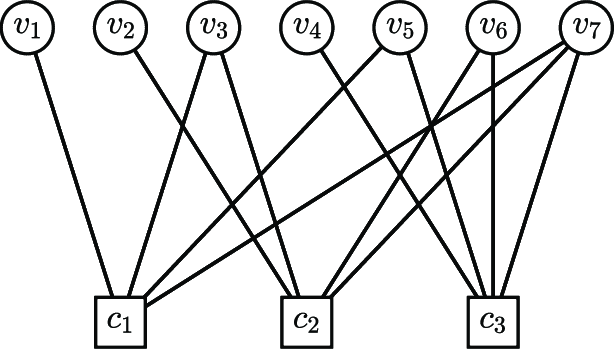
\includegraphics[scale=0.5]{Tanner1.png}  
  \caption{Graphe de Tanner associé}
  \label{fig:Tanner1}
\end{figure}
\clearpage
\textbf{Autre exemple:}
Soit la matrice de Parité : \newline
$$H=
\begin{pmatrix}
  1 & 0 & 0 & 0 & 1 & 0 & 0 & 0 \\
  0 & 1 & 0 & 0 & 1 & 1 & 0 & 0 \\
  
  0 & 0 & 1 & 0 & 0 & 1 & 1 & 0 \\
  0 & 0 & 0 & 1 & 0 & 0 & 1 & 1 
  
  
\end{pmatrix}
\quad
$$
\begin{figure}[!h]
  \centering
  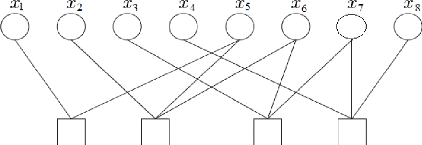
\includegraphics[scale=0.5]{Tanner2.png}  
  \caption{Graphe biparti de Tanner associé}
  \label{fig:Tanner2}
\end{figure}

Le graphe de Tanner est utilisé comme support pour la plupart des algorithmes de décodage. Le principe principal d'un algorithme de décodage utilisant cette 
représentation est de considérer chaque branche du graphe comme un message d'un noeud $c_j$ vers un noeud $v_i$ et réciproquement.

%\subsection{Vocabulaire}
\newpage
%-----------------------------------------------------
%-----------------------------------------------------

\section{Algorithme de décodage}
\label{sec:algo}
Il existe plusieurs types d'algorithmes de décodage pour les codes LDPC. Cependant, nous en avons étudier un seul.
Ce dernier consiste à faire baisser le poids du syndrome jusqu'à que ce dernier soit nul. L'objectif de cet algorithme 
est de relever les colonnes d'une matrice de parité $H$ qui sont erronés.
Pour ce faire, les positions qui sont en erreurs vont faire baisser le poids de notre syndrome. Ainsi, on va parcourir 
chaque colonnes de la matrice $H$ afin de trouver ces dernières.
On définit le code LDPC $C$ à l'aide d'une matrice de parité \textbf{H}, qui est creuse.
Soit $y = x + e$, où $y$ est le message reçu, $x$ le message chiffré et $e$ le vecteur erreur.\vspace{0.4cm}\newline

Voici l'algorithme:\vspace{0.4cm}\newline

\begin{algorithm}[H]
  \SetAlgoLined
  \KwData{Soient $E$ un motif d'erreur et $H$ une matrice de parité de taille $n$. }
  \KwResult{Syndrome de l'erreur courant}

  On définit les $h_{i}$, $\forall i \in \llbracket 0~;~ n \rrbracket$ les colonnes de la matrice H.
  
  Et on note $\omega(e)$ le poids de $e$.

  $S = \sigma(E) = H.~^tE$
  
  %$compteur \leftarrow 0$

  \For{$i\leftarrow 0$ \KwTo $n$}{
     \If{$\omega(S + h_{i}) \le \omega(S)$}{
      $E_1 \leftarrow E_1 + h_i$ 
    }
  }
  \eIf{$S = \omega(E_1)$}{
    le syndrome de l'erreur trouvé est le syndrome de l'erreur courante\;
    \KwRet{$E_1$}
  }{
    on répète l'algorithme avec le nouveau motif d'erreur trouvé\;
    $S = \sigma(E) + \sigma(E_1) = \sigma(E + E_1)$\;
    \KwRet{$E_1 + $} \Repeat{$\omega(S) = 0$}{}
  }
  \caption{Algorithme de décodage LDPC}
\end{algorithm}
\vspace{0.4cm}
On peut remarquer que l'algorithme peut vite faire une boucle infini si la condition à la ligne 
\textbf{\textsc{17}} n'est pas satisfaite.
Nous allons définir un nombre maximal d'itération à exécuter. En effet, il se peut que l'algorithme 
de décodage LDPC ne trouve pas de solution, de ce faite, on évite une boucle infini.\vspace{0.4cm}\newline
Dans notre implémentation Python, nous avons fait le choix d'éxécuter au plus 25 fois la recherche puisque 
si le poids ne diminue plus, on ne peut pas décoder le code LDPC. Nous verrons cela dans la partie \ref{sec:exp}.
\clearpage
\lstinputlisting[language=python, firstline=7, lastline=41]{main.py}
\vspace{0.5cm} Les fonctions auxiliaires apparaissent sur l'annexe \ref{sec:annexe}.
%Pour écrire des algorithmes, le paquetage suivant est très utile : \url{http://tug.ctan.org/macros/latex/contrib/algorithm2e/doc/algorithm2e.pdf}  
\clearpage
%-----------------------------------------------------
%-----------------------------------------------------

\section{Expérimentations et résultats}
\label{sec:exp}

Nous avons réaliser plusieurs types d'expériences. Nous avons découvert que plus la taille des matrices est grandes, 
plus l'algorithme de décodage fonctionne. En effet, Pour livrer nos résultats, nous avons choisit des matrices de longueur 
$1000$ et $2000$.

Nous avons implémenter des fonctions\ref{sec:annexe} de façon à pouvoir créer des matrices creuses.
La fonction \textit{matrixFromWeight(poids,n)} créer une matrice de dimension $\dfrac{n}{2}$ par $n$ de tel sorte que 
chaque colonne est un poids de valeur $poids$ et est unique. Sinon, notre matrice de parité ne représente pas un code LDPC régulier.\vspace{0.4cm}\newline
\underline{Objectif de l'expérimentation:} Nous allons essayer de déterminer le poids optimale sur chaque colonne pour décoder un code 
LDPC de longueur $n$.\vspace{0.4cm}\newline
La méthode adopter est la suivante:
\begin{enumerate}
  \item[1.] Construire une matrice dont les colonnes ont un certain poids.
  \item[2.] Observer combien de vecteurs erreurs d'un certain poids, nous arrivons à retrouver grâce à notre algorithme de décodage classique.
  \item[3.] Essayer d'optimiser l'algorithme de décodage en supprimant les position parasites et donc essayer de décoder plus de vecteurs erreurs.
  \item[4.] Comparer les résultats des deux algorithmes.
\end{enumerate}

\textsc{\textbf{\underline{Remarque :}}} Une position parasite est une colonne de H qui satisfait la condition\newline $\omega(S + h_{i}) \le \omega(S)(1)$ mais qui n'est pas une 
position érroné. En outre, on va durcir la condition $(1)$ de façon a ignorer ces positions. Pour cela, on essaiera de récupérer les colonnes de H qui font baisser le
syndrome. ($\omega(S + h_{i}) < \omega(S)$ ou encore $\omega(S + h_{i}) < \omega(S) - 1$, par exemple)

\subsection{$n = 1000$}
Nous réalisons 

\textbf{\underline{Nota bene:}} 



La Table \ref{table:resultats} présente un résumé des résultats de nos expérimentations. 

\begin{table}[htbp]
  \centering
  \caption{Comparaison des différentes méthodes}
  \label{table:resultats}
    \begin{tabular}{l|rrrrr}
    \hline
    \multirow{2}[0]{*}{Algorithme}&  \multicolumn{2}{c}{Temps CPU (ms)}  & \multicolumn{2}{c}{Gap MS} &  \multirow{2}[0]{*}{\#Données MS}  \\
        & \multicolumn{1}{c}{Moyenne}   & \multicolumn{1}{c}{Ecart type} & \multicolumn{1}{c}{Moyenne} & \multicolumn{1}{c}{Ecart type} & \\
          \hline
    Heuristique PPV & 29 & 96 & 8.4\% & \textbf{36\%} &  6/38\\
    Heuristique MI & 16984 & 78093  & \textbf{1.3\%} & 42\% &   \textbf{30/38} \\
    \hline
    \end{tabular}%
\end{table}%

\FloatBarrier
\clearpage
%-----------------------------------------------------
%-----------------------------------------------------

\section{Conclusion}
\label{sec:conclusion}
C'est la fin.

\clearpage

%% Les appendices commencent après la commande \appendix
%% Les commandes \chapter (si l'option chapter est sélectionnée), \section, \subsection peuvent s'utiliser comme habituellement
%\appendix

%\clearpage % à utiliser pour afficher la biblographie sur une nouvelle page
% References

%\printbibliography
\section{Annexe}
\label{sec:annexe}
\underline{Fichier tools.py}
\lstinputlisting[language=python]{tools.py}
\mbox{}\hfill\rule{0.5\linewidth}{1mm}\hfill\mbox{}
\vspace{0.3cm}\newline
\underline{Fichier matrix.py}
\lstinputlisting[language=python]{matrix.py}
\mbox{}\hfill\rule{0.5\linewidth}{1mm}\hfill\mbox{}
\vspace{0.3cm}\newline
\underline{Fichier main.py}
\lstinputlisting[language=python]{main.py}


\end{document}
